\documentclass[a4paper,12pt]{paper}

\usepackage{mycommands}

% Worked-example layout: boxed problem statement followed by a solution.
\newcounter{example}
\renewenvironment{example}[1]{%  % the paper class already defines "example"
  \refstepcounter{example}%
  \begin{mdframed}[linewidth=1pt,innertopmargin=6pt,innerbottommargin=6pt]%
  \noindent\textbf{Example \theexample: #1.}\ }{%
  \end{mdframed}}
\newenvironment{solution}{\par\noindent\textbf{Solution.}\ }{\par\medskip}

\title{Worked examples for Lecture 22: Free oscillations}
\author{David Al-Attar \\ Michaelmas Term, \the\year}

\begin{document}

\maketitle

\noindent These examples accompany Lecture~22. They are intended as practice in the concrete
calculations that underlie the lecture, and are less demanding than the questions on the
problem sets. Numerical results were checked with the scripts in the \texttt{python}
directory.

%----------------------------------------------------------------------------------------
\begin{example}{A two-degree-of-freedom analogue}
Two particles of mass $m$ and $2m$ move along a line. The first is attached to a fixed wall
by a spring of stiffness $k$, the two particles are joined by a spring of stiffness $2k$, and
the second is attached to a second fixed wall by a spring of stiffness $2k$. Let $u_{1}(t)$
and $u_{2}(t)$ be the displacements from equilibrium, and let external forces $f_{1}(t)$ and
$f_{2}(t)$ act on the particles. (a)~Write the equations of motion in the form
$\mathbf{M}\ddot{\mathbf{u}}+\mathbf{K}\mathbf{u}=\mathbf{f}$. (b)~Find the eigenfrequencies
and eigenvectors, show that the eigenvectors are orthogonal with respect to $\mathbf{M}$, and
normalise them so that $\mathbf{s}_{k}^{T}\mathbf{M}\mathbf{s}_{k}=1$. (c)~Show that in the
frequency domain
$\tilde{\mathbf{u}}=\sum_{k}\frac{\mathbf{s}_{k}(\mathbf{s}_{k}^{T}\tilde{\mathbf{f}})}{\omega_{k}^{2}-\omega^{2}}$.
(d)~For the step force $\mathbf{f}(t)=(0,F_{0})^{T}H(t)$, with $H$ the Heaviside function,
obtain the time-domain solution and check its long-time average against the static solution.
\end{example}

\begin{solution}
(a) The spring forces on the first particle are $-ku_{1}$ from the wall spring and
$-2k(u_{1}-u_{2})$ from the coupling spring, while the second particle feels $-2k(u_{2}-u_{1})$
and $-2ku_{2}$. Newton's second law therefore gives
\begin{equation}
\begin{pmatrix} m & 0 \\ 0 & 2m\end{pmatrix}
\begin{pmatrix}\ddot{u}_{1}\\ \ddot{u}_{2}\end{pmatrix}
+k\begin{pmatrix} 3 & -2 \\ -2 & 4\end{pmatrix}
\begin{pmatrix}u_{1}\\ u_{2}\end{pmatrix}
=\begin{pmatrix}f_{1}\\ f_{2}\end{pmatrix},
\label{eq:1}
\end{equation}
which defines $\mathbf{M}$ and $\mathbf{K}$. Both matrices are symmetric, and both are positive
definite. This is the finite-dimensional counterpart of the weak form
$\langle\mathbf{w}|P|\ddot{\mathbf{u}}\rangle+\langle\mathbf{w}|H|\mathbf{u}\rangle=\langle\mathbf{w}|\mathbf{f}\rangle$
in the lecture, with the correspondences
$\langle\mathbf{w}|P|\mathbf{u}\rangle\leftrightarrow\mathbf{w}^{T}\mathbf{M}\mathbf{u}$,
$\langle\mathbf{w}|H|\mathbf{u}\rangle\leftrightarrow\mathbf{w}^{T}\mathbf{K}\mathbf{u}$ and
$\langle\mathbf{w}|\mathbf{f}\rangle\leftrightarrow\mathbf{w}^{T}\mathbf{f}$. Since everything
is real we can work with real vectors, and the symmetry of $\mathbf{M}$ and $\mathbf{K}$ is
the analogue of the self-adjointness of the kinetic and potential energy forms.

(b) Substituting $\mathbf{u}=\mathbf{s}\ee^{\ii\omega t}$ with $\mathbf{f}=\mathbf{0}$ gives the
generalised eigenvalue problem $\mathbf{K}\mathbf{s}=\omega^{2}\mathbf{M}\mathbf{s}$. Non-trivial
solutions require
\begin{equation}
\det(\mathbf{K}-\omega^{2}\mathbf{M})=(3k-m\omega^{2})(4k-2m\omega^{2})-4k^{2}
=2(m\omega^{2}-k)(m\omega^{2}-4k)=0,
\label{eq:2}
\end{equation}
so that the squared eigenfrequencies are $\omega_{1}^{2}=k/m$ and $\omega_{2}^{2}=4k/m$. For
$\omega_{1}^{2}$ the matrix $\mathbf{K}-\omega_{1}^{2}\mathbf{M}$ has rows proportional to
$(1,-1)$, giving $\mathbf{s}_{1}\propto(1,1)^{T}$; for $\omega_{2}^{2}$ the rows are proportional
to $(1,2)$, giving $\mathbf{s}_{2}\propto(2,-1)^{T}$. The mass-weighted inner product of these
vectors is $m(1\times 2)+2m(1\times(-1))=0$, so they are $\mathbf{M}$-orthogonal even though they
are not orthogonal in the usual sense. This is a general fact: from
$\mathbf{s}_{2}^{T}\mathbf{K}\mathbf{s}_{1}=\omega_{1}^{2}\mathbf{s}_{2}^{T}\mathbf{M}\mathbf{s}_{1}$
and $\mathbf{s}_{1}^{T}\mathbf{K}\mathbf{s}_{2}=\omega_{2}^{2}\mathbf{s}_{1}^{T}\mathbf{M}\mathbf{s}_{2}$,
the symmetry of $\mathbf{K}$ and $\mathbf{M}$ shows that the left-hand sides are equal, and hence
$(\omega_{1}^{2}-\omega_{2}^{2})\,\mathbf{s}_{1}^{T}\mathbf{M}\mathbf{s}_{2}=0$, exactly as in the
lecture. Normalising, we take
\begin{equation}
\mathbf{s}_{1}=\frac{1}{\sqrt{3m}}\begin{pmatrix}1\\1\end{pmatrix},\quad
\mathbf{s}_{2}=\frac{1}{\sqrt{6m}}\begin{pmatrix}2\\-1\end{pmatrix},\quad
\mathbf{s}_{j}^{T}\mathbf{M}\mathbf{s}_{k}=\delta_{jk}.
\label{eq:3}
\end{equation}
Because the two eigenvectors are linearly independent, any vector can be expanded as
$\mathbf{u}=\sum_{k}(\mathbf{s}_{k}^{T}\mathbf{M}\mathbf{u})\mathbf{s}_{k}$, which is the
two-dimensional version of the completeness relation in the lecture.

(c) With the transform convention of the lecture,
$\tilde{\mathbf{u}}(\omega)=\int_{0}^{\infty}\mathbf{u}(t)\ee^{-\ii\omega t}\dd t$, and zero
initial conditions, two integrations by parts give
$\widetilde{\ddot{\mathbf{u}}}=-\omega^{2}\tilde{\mathbf{u}}$, and so
$-\omega^{2}\mathbf{M}\tilde{\mathbf{u}}+\mathbf{K}\tilde{\mathbf{u}}=\tilde{\mathbf{f}}$.
Writing $\tilde{\mathbf{u}}=\sum_{k}c_{k}\mathbf{s}_{k}$, using
$\mathbf{K}\mathbf{s}_{k}=\omega_{k}^{2}\mathbf{M}\mathbf{s}_{k}$, and premultiplying by
$\mathbf{s}_{j}^{T}$, we find that $(\omega_{j}^{2}-\omega^{2})c_{j}=\mathbf{s}_{j}^{T}\tilde{\mathbf{f}}$,
and so
\begin{equation}
\tilde{\mathbf{u}}(\omega)=\sum_{k=1}^{2}\frac{\mathbf{s}_{k}(\mathbf{s}_{k}^{T}\tilde{\mathbf{f}})}{\omega_{k}^{2}-\omega^{2}},
\label{eq:4}
\end{equation}
which is the eigenfunction expansion solution of the lecture with the bra-kets replaced by matrix
products. The resonances at $\omega=\pm\omega_{k}$ are evident.

(d) The time-domain solution is easiest to obtain by projecting the equations of motion rather
than by inverting eq.~(\ref{eq:4}). Let $q_{k}(t)=\mathbf{s}_{k}^{T}\mathbf{M}\mathbf{u}(t)$ be the
modal coordinates, so that $\mathbf{u}=\sum_{k}q_{k}\mathbf{s}_{k}$. Premultiplying
eq.~(\ref{eq:1}) by $\mathbf{s}_{k}^{T}$, and using the transposed eigenvalue equation
$\mathbf{s}_{k}^{T}\mathbf{K}=\omega_{k}^{2}\mathbf{s}_{k}^{T}\mathbf{M}$, we obtain the
uncoupled oscillator equations
\begin{equation}
\ddot{q}_{k}+\omega_{k}^{2}q_{k}=\mathbf{s}_{k}^{T}\mathbf{f}(t),\quad q_{k}(0)=\dot{q}_{k}(0)=0.
\label{eq:5}
\end{equation}
For the step force $\mathbf{s}_{k}^{T}\mathbf{f}=F_{k}H(t)$ with $F_{k}=\mathbf{s}_{k}^{T}(0,F_{0})^{T}$
constant, and one checks by differentiation that the solution for $t>0$ is
\begin{equation}
q_{k}(t)=F_{k}\,\frac{1-\cos\omega_{k}t}{\omega_{k}^{2}},
\label{eq:6}
\end{equation}
since $\ddot{q}_{k}=F_{k}\cos\omega_{k}t$ and hence $\ddot{q}_{k}+\omega_{k}^{2}q_{k}=F_{k}$,
while $q_{k}$ and $\dot{q}_{k}=F_{k}\sin(\omega_{k}t)/\omega_{k}$ both vanish at $t=0$. Here
$F_{1}=F_{0}/\sqrt{3m}$ and $F_{2}=-F_{0}/\sqrt{6m}$, so with $\omega_{2}=2\omega_{1}$ we find
\begin{align}
u_{1}(t)&=\frac{F_{0}}{3k}(1-\cos\omega_{1}t)-\frac{F_{0}}{12k}(1-\cos 2\omega_{1}t),\nonumber\\
u_{2}(t)&=\frac{F_{0}}{3k}(1-\cos\omega_{1}t)+\frac{F_{0}}{24k}(1-\cos 2\omega_{1}t).
\label{eq:7}
\end{align}
Averaging over the common period $2\pi/\omega_{1}$ replaces each factor $1-\cos\omega_{k}t$
by unity, and gives $\bar{u}_{1}=F_{0}/4k$ and $\bar{u}_{2}=3F_{0}/8k$; these are exactly the
components of the static solution $\mathbf{K}^{-1}(0,F_{0})^{T}$, as they should be. The response is the static
deflection plus an undamped oscillation about it, and since $\omega_{2}=2\omega_{1}$ the motion
here is periodic.
As a consistency check on eq.~(\ref{eq:4}), note that for $\mathrm{Im}\,\omega<0$ the transform of
$H(t)$ is $1/(\ii\omega)$, while
\begin{equation}
\int_{0}^{\infty}\frac{1-\cos\omega_{k}t}{\omega_{k}^{2}}\ee^{-\ii\omega t}\dd t
=\frac{1}{\omega_{k}^{2}}\left(\frac{1}{\ii\omega}-\frac{\ii\omega}{\omega_{k}^{2}-\omega^{2}}\right)
=\frac{1}{\ii\omega(\omega_{k}^{2}-\omega^{2})},
\label{eq:8}
\end{equation}
so the transform of eq.~(\ref{eq:6}) is precisely $F_{k}\tilde{H}(\omega)/(\omega_{k}^{2}-\omega^{2})$,
the $k$th coefficient in eq.~(\ref{eq:4}). Everything in the lecture's derivation, including the
$\frac{1-\cos\omega_{k}t}{\omega_{k}^{2}}$ time dependence used in the second problem set, is already
present in this two-dimensional model; the continuum case differs only in having infinitely many modes.
\end{solution}

%----------------------------------------------------------------------------------------
\begin{example}{A free--free rod}
A uniform elastic rod of density $\rho$ and Young's modulus $E$ occupies $0\le x\le L$ and has
traction-free ends. Its longitudinal displacement $u(x,t)$ satisfies
$\rho\ddot{u}-E u''=-\partial_{x}\overline{S}$ with $Eu'=\overline{S}$ at $x=0,L$, where
$\overline{S}(x,t)$ is a stress glut. (a)~Write down the weak form and the normalised eigenfunctions
$|k\rangle$ and eigenfrequencies $\omega_{k}$. (b)~Show that the rigid-translation mode $k=0$ is
not excited by any stress glut. (c)~For the point source $\overline{S}=M_{0}\delta(x-x_{s})H(t)$ with
$0<x_{s}<L$, write down the response using the time-domain mode sum of the second problem set, check
the initial conditions and, by direct substitution, the equation of motion, and interpret the
long-time average of the solution.
\end{example}

\begin{solution}
(a) Multiplying the equation of motion by a test function $w^{*}$, integrating over the rod, and
integrating by parts using the boundary condition $Eu'-\overline{S}=0$ at the ends gives
\begin{equation}
\int_{0}^{L}\rho w^{*}\ddot{u}\dd x+\int_{0}^{L}E\,\frac{\partial w^{*}}{\partial x}\frac{\partial u}{\partial x}\dd x
=\int_{0}^{L}\overline{S}\,\frac{\partial w^{*}}{\partial x}\dd x,
\label{eq:9}
\end{equation}
which is $\langle w|P|\ddot{u}\rangle+\langle w|H|u\rangle=\langle w|f\rangle$ in one dimension.
Time-harmonic free solutions $s(x)\ee^{\ii\omega t}$ satisfy $Es''=-\omega^{2}\rho s$ with
$s'(0)=s'(L)=0$, so $s\propto\cos(k\pi x/L)$ with $k=0,1,2,\dots$ and
\begin{equation}
\omega_{k}=\frac{k\pi c}{L},\quad c=\sqrt{\frac{E}{\rho}}.
\label{eq:10}
\end{equation}
Since $\int_{0}^{L}\cos^{2}(k\pi x/L)\dd x=L/2$ for $k\ge 1$ and $L$ for $k=0$, the
eigenfunctions normalised by $\langle k|P|k'\rangle=\int_{0}^{L}\rho\,|k\rangle|k'\rangle\dd x=\delta_{kk'}$ are
\begin{equation}
|0\rangle=\frac{1}{\sqrt{\rho L}},\quad
|k\rangle=\sqrt{\frac{2}{\rho L}}\cos\frac{k\pi x}{L}\quad(k\ge 1).
\label{eq:11}
\end{equation}
Each eigenspace is one-dimensional, so the second label $m$ of the lecture is not needed.

(b) The force term for the $k$th mode is $\langle k|f\rangle=\int_{0}^{L}\overline{S}\,\partial_{x}|k\rangle\dd x$.
For $k=0$ the eigenfunction is constant, its derivative vanishes, and so $\langle 0|f\rangle=0$
whatever $\overline{S}$ may be. This is the one-dimensional version of the lecture's statement that
the trivial modes cannot be excited by a seismic source: an internal source exerts no net force,
and the centre of mass, $\int_{0}^{L}\rho u\dd x\propto\langle 0|P|u\rangle$, remains at rest.

(c) For the point source, $\langle k|f\rangle(t)=M_{0}H(t)\,\partial_{x}|k\rangle(x_{s})=F_{k}H(t)$ with
\begin{equation}
F_{k}=-M_{0}\sqrt{\frac{2}{\rho L}}\,\frac{k\pi}{L}\sin\frac{k\pi x_{s}}{L}.
\label{eq:12}
\end{equation}
The mode sum from the second problem set requires the time integrals
$\int_{0}^{t}\sin[\omega_{k}(t-t')]\,H(t')\dd t'/\omega_{k}=(1-\cos\omega_{k}t)/\omega_{k}^{2}$, and so
\begin{equation}
u(x,t)=\sum_{k=1}^{\infty}F_{k}\frac{1-\cos\omega_{k}t}{\omega_{k}^{2}}|k\rangle(x)
=-\frac{2M_{0}}{\pi E}\sum_{k=1}^{\infty}\frac{1}{k}\sin\frac{k\pi x_{s}}{L}\cos\frac{k\pi x}{L}
\left(1-\cos\frac{k\pi ct}{L}\right),
\label{eq:13}
\end{equation}
where we used $\omega_{k}^{2}=Ek^{2}\pi^{2}/(\rho L^{2})$ to simplify the coefficients. At $t=0$
every term vanishes, and the time derivative brings down a factor $\omega_{k}\sin\omega_{k}t$ that
also vanishes, so $u(x,0)=\dot{u}(x,0)=0$ as required. The boundary conditions hold term by term,
since $\partial_{x}\cos(k\pi x/L)$ vanishes at both ends, in agreement with $Eu'=\overline{S}=0$ there.

For the direct substitution we apply $\rho\partial_{t}^{2}-E\partial_{x}^{2}$ to each term of
eq.~(\ref{eq:13}). Since $E(k\pi/L)^{2}=\rho\omega_{k}^{2}$, the $k$th term is multiplied by
$\rho\omega_{k}^{2}[\cos\omega_{k}t+(1-\cos\omega_{k}t)]=\rho\omega_{k}^{2}$ for $t>0$, so
\begin{equation}
\rho\ddot{u}-Eu''=-\frac{2M_{0}}{\pi E}\sum_{k=1}^{\infty}\frac{\rho\omega_{k}^{2}}{k}\sin\frac{k\pi x_{s}}{L}\cos\frac{k\pi x}{L}
=-\frac{2\pi M_{0}}{L^{2}}\sum_{k=1}^{\infty}k\sin\frac{k\pi x_{s}}{L}\cos\frac{k\pi x}{L}.
\label{eq:14}
\end{equation}
To identify the right-hand side we use the completeness relation,
$u(x)=\sum_{k}\langle k|P|u\rangle|k\rangle$, which on writing out the inner product becomes
$\rho\sum_{k}|k\rangle(x)|k\rangle(x')=\delta(x-x')$, and which, with eq.~(\ref{eq:11}), is the
cosine series
\begin{equation}
\delta(x-x_{s})=\frac{1}{L}+\frac{2}{L}\sum_{k=1}^{\infty}\cos\frac{k\pi x_{s}}{L}\cos\frac{k\pi x}{L}.
\label{eq:15}
\end{equation}
Differentiating with respect to $x_{s}$, and using $\partial_{x_{s}}\delta(x-x_{s})=-\delta'(x-x_{s})$, gives
\begin{equation}
\delta'(x-x_{s})=\frac{2\pi}{L^{2}}\sum_{k=1}^{\infty}k\sin\frac{k\pi x_{s}}{L}\cos\frac{k\pi x}{L},
\label{eq:16}
\end{equation}
and comparison with eq.~(\ref{eq:14}) shows that
$\rho\ddot{u}-Eu''=-M_{0}\delta'(x-x_{s})H(t)=-\partial_{x}\overline{S}$, as required. The series in
eqs.~(\ref{eq:15}) and (\ref{eq:16}) converge only in the sense of distributions, which is the sense in
which a point source satisfies the equation of motion; the series in eq.~(\ref{eq:13}) for the
displacement itself has coefficients decaying like $1/k$ and converges, though slowly, to a function
with a jump.

That jump is the physical content of the long-time average. Averaging over time replaces each
$1-\cos\omega_{k}t$ by $1$, and the resulting series is the cosine series of the static solution.
Indeed, the static problem $Eu'=\overline{S}$ integrates to $u=(M_{0}/E)H(x-x_{s})+\mathrm{const}$,
and the constant is fixed by $\langle 0|P|u\rangle=0$, i.e.\ zero mean displacement. The function
$g(x)=(M_{0}/E)[H(x-x_{s})-(L-x_{s})/L]$ has $\int_{0}^{L}g\dd x=0$ and cosine coefficients
\begin{equation}
\frac{2}{L}\int_{0}^{L}g(x)\cos\frac{k\pi x}{L}\dd x=\frac{2M_{0}}{EL}\int_{x_{s}}^{L}\cos\frac{k\pi x}{L}\dd x
=-\frac{2M_{0}}{\pi Ek}\sin\frac{k\pi x_{s}}{L},
\label{eq:17}
\end{equation}
which are exactly the time-averaged coefficients in eq.~(\ref{eq:13}). The point stress glut is
therefore a dislocation: the material on the two sides of $x_{s}$ is permanently offset by $M_{0}/E$,
the mean displacement stays zero, and the dynamic solution consists of the waves radiated by the sudden
appearance of this offset, reflecting for ever between the free ends because we have neglected attenuation.
Numerically, a partial sum with $20\,000$ terms reproduces the step to four decimal places away from
$x_{s}$, and the mode sum for a Gaussian-smoothed glut agrees with a finite-difference solution of the rod
to the discretisation error of the latter.
\end{solution}

%----------------------------------------------------------------------------------------
\begin{example}{Verifying the time-domain mode sum}
The second problem set quotes the time-domain solution of the forced problem in a non-rotating earth
model,
\begin{equation}
\mathbf{u}(\mathbf{x},t)=\sum_{km}\left\{\int_{0}^{t}\frac{\sin[\omega_{k}(t-t')]}{\omega_{k}}
\int_{M}\overline{S}_{ij}(\mathbf{x}',t')\frac{\partial|km\rangle^{*}}{\partial x'_{j}}(\mathbf{x}')\dd^{3}\mathbf{x}'\dd t'\right\}|km\rangle(\mathbf{x}).
\label{eq:18}
\end{equation}
Show by direct substitution that this satisfies the weak form
$\langle\mathbf{w}|P|\ddot{\mathbf{u}}\rangle+\langle\mathbf{w}|H|\mathbf{u}\rangle=\langle\mathbf{w}|\mathbf{f}\rangle$
for every test function $\mathbf{w}$, together with the initial conditions
$\mathbf{u}(\mathbf{x},0)=\dot{\mathbf{u}}(\mathbf{x},0)=\mathbf{0}$. Then show that its Fourier transform
is the frequency-domain eigenfunction expansion of the lecture, and specialise to a source that is a step
in time, $\overline{S}_{ij}(\mathbf{x},t)=\overline{S}_{ij}(\mathbf{x})H(t)$.
\end{example}

\begin{solution}
The inner spatial integral in eq.~(\ref{eq:18}) is the force term of the lecture evaluated on the
$(k,m)$th eigenfunction,
\begin{equation}
F_{km}(t)=\langle km|\mathbf{f}\rangle(t)=\int_{M}\overline{S}_{ij}(\mathbf{x},t)\frac{\partial|km\rangle_{i}^{*}}{\partial x_{j}}\dd^{3}\mathbf{x},
\label{eq:19}
\end{equation}
so that eq.~(\ref{eq:18}) reads $\mathbf{u}=\sum_{km}q_{km}(t)|km\rangle$ with the modal coordinates
\begin{equation}
q_{km}(t)=\int_{0}^{t}\frac{\sin[\omega_{k}(t-t')]}{\omega_{k}}F_{km}(t')\dd t'.
\label{eq:20}
\end{equation}
A word about the trivial modes. If $\omega_{k}=0$ then $\sin[\omega_{k}(t-t')]/\omega_{k}$ is to be read
as its limit $t-t'$, but for these modes $|km\rangle_{i}=a_{i}+B_{ij}x_{j}$ with $B_{ij}$ anti-symmetric,
so $\partial_{j}|km\rangle_{i}=B_{ij}$, and its contraction with the symmetric $\overline{S}_{ij}$ in
eq.~(\ref{eq:19}) vanishes. The trivial modes therefore contribute nothing, and in what follows we
may take $\omega_{k}>0$.

Differentiating eq.~(\ref{eq:20}) with respect to its upper limit and under the integral sign,
\begin{equation}
\dot{q}_{km}(t)=\frac{\sin 0}{\omega_{k}}F_{km}(t)+\int_{0}^{t}\cos[\omega_{k}(t-t')]F_{km}(t')\dd t'
=\int_{0}^{t}\cos[\omega_{k}(t-t')]F_{km}(t')\dd t',
\label{eq:21}
\end{equation}
and differentiating once more,
\begin{equation}
\ddot{q}_{km}(t)=F_{km}(t)-\omega_{k}\int_{0}^{t}\sin[\omega_{k}(t-t')]F_{km}(t')\dd t'
=F_{km}(t)-\omega_{k}^{2}q_{km}(t).
\label{eq:22}
\end{equation}
Thus each modal coordinate satisfies the forced oscillator equation
$\ddot{q}_{km}+\omega_{k}^{2}q_{km}=F_{km}$, and from eqs.~(\ref{eq:20}) and (\ref{eq:21}) both
$q_{km}(0)$ and $\dot{q}_{km}(0)$ vanish, since the integrals are over an interval of zero length.
Hence $\mathbf{u}(\mathbf{x},0)=\dot{\mathbf{u}}(\mathbf{x},0)=\mathbf{0}$. Eq.~(\ref{eq:20}) is just
Duhamel's formula for this oscillator.

Now substitute into the weak form, differentiating the sum term by term. Using the sesquilinearity of
the forms and the eigenvalue equation
$\langle\mathbf{w}|H|km\rangle=\omega_{k}^{2}\langle\mathbf{w}|P|km\rangle$, which holds for every test
function $\mathbf{w}$,
\begin{align}
\langle\mathbf{w}|P|\ddot{\mathbf{u}}\rangle+\langle\mathbf{w}|H|\mathbf{u}\rangle
&=\sum_{km}\left[\ddot{q}_{km}\langle\mathbf{w}|P|km\rangle+q_{km}\langle\mathbf{w}|H|km\rangle\right]\nonumber\\
&=\sum_{km}\left(\ddot{q}_{km}+\omega_{k}^{2}q_{km}\right)\langle\mathbf{w}|P|km\rangle
=\sum_{km}F_{km}\langle\mathbf{w}|P|km\rangle.
\label{eq:23}
\end{align}
It remains to identify the last sum with $\langle\mathbf{w}|\mathbf{f}\rangle$. Expanding the test
function using completeness, $\mathbf{w}=\sum_{km}\langle km|P|\mathbf{w}\rangle|km\rangle$, and
recalling that $\langle\mathbf{w}|\mathbf{f}\rangle$ is conjugate-linear in $\mathbf{w}$, we have
\begin{equation}
\langle\mathbf{w}|\mathbf{f}\rangle=\sum_{km}\langle km|P|\mathbf{w}\rangle^{*}\langle km|\mathbf{f}\rangle
=\sum_{km}\langle\mathbf{w}|P|km\rangle F_{km},
\label{eq:24}
\end{equation}
where the self-adjointness of the kinetic energy form,
$\langle km|P|\mathbf{w}\rangle^{*}=\langle\mathbf{w}|P|km\rangle$, was used in the last step.
Eqs.~(\ref{eq:23}) and (\ref{eq:24}) agree for every $\mathbf{w}$, so eq.~(\ref{eq:18}) solves the
weak form, and because the weak form incorporates the boundary conditions, the traction condition on
$\partial M$ is satisfied automatically by the eigenfunctions. Only three ingredients were needed:
the eigenvalue equation, the orthonormality and completeness of the eigenfunctions, and the
self-adjointness of $P$.

For the connection with the frequency domain, we take the transform of eq.~(\ref{eq:20}),
namely $\tilde{q}_{km}(\omega)=\int_{0}^{\infty}q_{km}\,\ee^{-\ii\omega t}\dd t$. Writing the exponential
as $\ee^{-\ii\omega(t-t')}\ee^{-\ii\omega t'}$ and exchanging the order of integration over the
region $0\le t'\le t<\infty$ gives the causal convolution theorem
$\tilde{q}_{km}=\tilde{g}_{k}\tilde{F}_{km}$ with
\begin{equation}
\tilde{g}_{k}(\omega)=\int_{0}^{\infty}\frac{\sin\omega_{k}t}{\omega_{k}}\ee^{-\ii\omega t}\dd t
=\frac{1}{2\ii\omega_{k}}\left[\frac{1}{\ii(\omega-\omega_{k})}-\frac{1}{\ii(\omega+\omega_{k})}\right]
=\frac{1}{\omega_{k}^{2}-\omega^{2}},
\label{eq:25}
\end{equation}
where the integral converges for $\mathrm{Im}\,\omega<0$, the standard device that corresponds physically
to a slight attenuation moving the poles off the real axis. Hence
\begin{equation}
\tilde{\mathbf{u}}=\sum_{km}\frac{\langle km|\tilde{\mathbf{f}}\rangle}{\omega_{k}^{2}-\omega^{2}}|km\rangle,
\label{eq:26}
\end{equation}
which is the eigenfunction expansion solution derived in the lecture; eq.~(\ref{eq:18}) is its inverse
transform, and the contour integration mentioned in the lecture simply evaluates the residues at
$\omega=\pm\omega_{k}$ to produce $\sin(\omega_{k}t)/\omega_{k}$. Finally, for a step-in-time source
$F_{km}(t)=F_{km}H(t)$ with $F_{km}=\int_{M}\overline{S}_{ij}(\mathbf{x})\partial_{j}|km\rangle_{i}^{*}\dd^{3}\mathbf{x}$
constant, the time integral in eq.~(\ref{eq:20}) is elementary and
\begin{equation}
\mathbf{u}(\mathbf{x},t)=\sum_{km}F_{km}\frac{1-\cos\omega_{k}t}{\omega_{k}^{2}}|km\rangle(\mathbf{x}),
\label{eq:27}
\end{equation}
the form used in Examples~1 and 2. Each mode is then displaced to a new static equilibrium
$F_{km}/\omega_{k}^{2}$ about which it oscillates for ever with amplitude equal to that offset, which is why
a step source excites the gravest modes, with the smallest $\omega_{k}^{2}$, so strongly.
\end{solution}

%----------------------------------------------------------------------------------------
\begin{example}{Spectral resolution and record length}
A seismogram is recorded for a time $T$, which we model by the boxcar window $h(t)=1$ for
$0\le t\le T$ and $h(t)=0$ otherwise. (a)~Compute $\tilde{h}(\omega)$, locate the first zero of
$|\tilde{h}|$ and find the full width at half maximum (FWHM) of the peak, both for the power spectrum
$|\tilde{h}|^{2}$ and the amplitude spectrum $|\tilde{h}|$. (b)~Show that the observed spectrum of an
undamped mode $u(t)=A\cos\omega_{0}t$ is a copy of $\tilde{h}$ centred on $\omega_{0}$, and state the
criterion for two modes with nearby frequencies to be resolved. (c)~The five singlets of the
multiplet $_{0}S_{2}$ are centred on $f_{0}\approx 0.3094\,\mathrm{mHz}$ and adjacent singlets are
separated by about $4.6\,\mu\mathrm{Hz}$. Estimate the record length needed to resolve them, and compare
it with the decay time of the mode, for which $Q\approx 510$.
\end{example}

\begin{solution}
(a) With the lecture's convention,
\begin{equation}
\tilde{h}(\omega)=\int_{0}^{T}\ee^{-\ii\omega t}\dd t=\frac{1-\ee^{-\ii\omega T}}{\ii\omega}
=T\ee^{-\ii\omega T/2}\,\frac{\sin(\omega T/2)}{\omega T/2},
\label{eq:28}
\end{equation}
so $|\tilde{h}(\omega)|=T|\mathrm{sinc}(\omega T/2)|$ with $\mathrm{sinc}\,x=\sin x/x$. In terms of the
frequency $f=\omega/2\pi$ the argument is $x=\pi fT$, and the zeros of $|\tilde{h}|$ lie at $f=n/T$ for
$n=\pm 1,\pm 2,\dots$; the first zero is at $f=1/T$. The power spectrum $|\tilde{h}|^{2}=T^{2}\mathrm{sinc}^{2}x$
falls to half its peak value where $\sin x/x=1/\sqrt{2}$, which has the root $x_{1/2}=1.3916$, and the
full width of the peak is therefore $2x_{1/2}/\pi$ in units of $1/T$:
\begin{equation}
\Delta f_{\mathrm{FWHM}}\left(|\tilde{h}|^{2}\right)=\frac{2x_{1/2}}{\pi T}=\frac{0.886}{T}.
\label{eq:29}
\end{equation}
For the amplitude spectrum the half-maximum condition is $\sin x/x=1/2$, with root $x=1.8955$, giving
$\Delta f_{\mathrm{FWHM}}(|\tilde{h}|)=1.207/T$. Whichever definition is used, the spectral line has a
width of order $1/T$, and the main lobe between the first zeros has total width $2/T$.

(b) A single undamped mode observed through the window has transform
\begin{equation}
\tilde{u}_{\mathrm{obs}}(\omega)=\int_{0}^{T}A\cos(\omega_{0}t)\ee^{-\ii\omega t}\dd t
=\frac{A}{2}\left[\tilde{h}(\omega-\omega_{0})+\tilde{h}(\omega+\omega_{0})\right],
\label{eq:30}
\end{equation}
which is the convolution result of the lecture made explicit: the transform of the infinite record,
with its poles at $\pm\omega_{0}$, is replaced by copies of $\tilde{h}$ centred on $\pm\omega_{0}$. Near
$\omega\approx\omega_{0}>0$ the second term is smaller by a factor of order $1/(\omega_{0}T)$ and can be
neglected whenever the record contains many cycles (for $_{0}S_{2}$ and $T=24\,\mathrm{h}$,
$\omega_{0}T\approx 170$). Two modes at $f_{1}$ and $f_{2}$ each contribute such a line, and by the
usual Rayleigh-type criterion they are resolved when the peak of one lies no closer than the first zero
of the other, i.e.\ when $|f_{1}-f_{2}|\gtrsim 1/T$. Fig.~\ref{fig:1} shows the amplitude spectrum of
two equal-amplitude cosines separated by $4.6\,\mu\mathrm{Hz}$ for two record lengths.

\begin{figure}[ht]
    \centering
    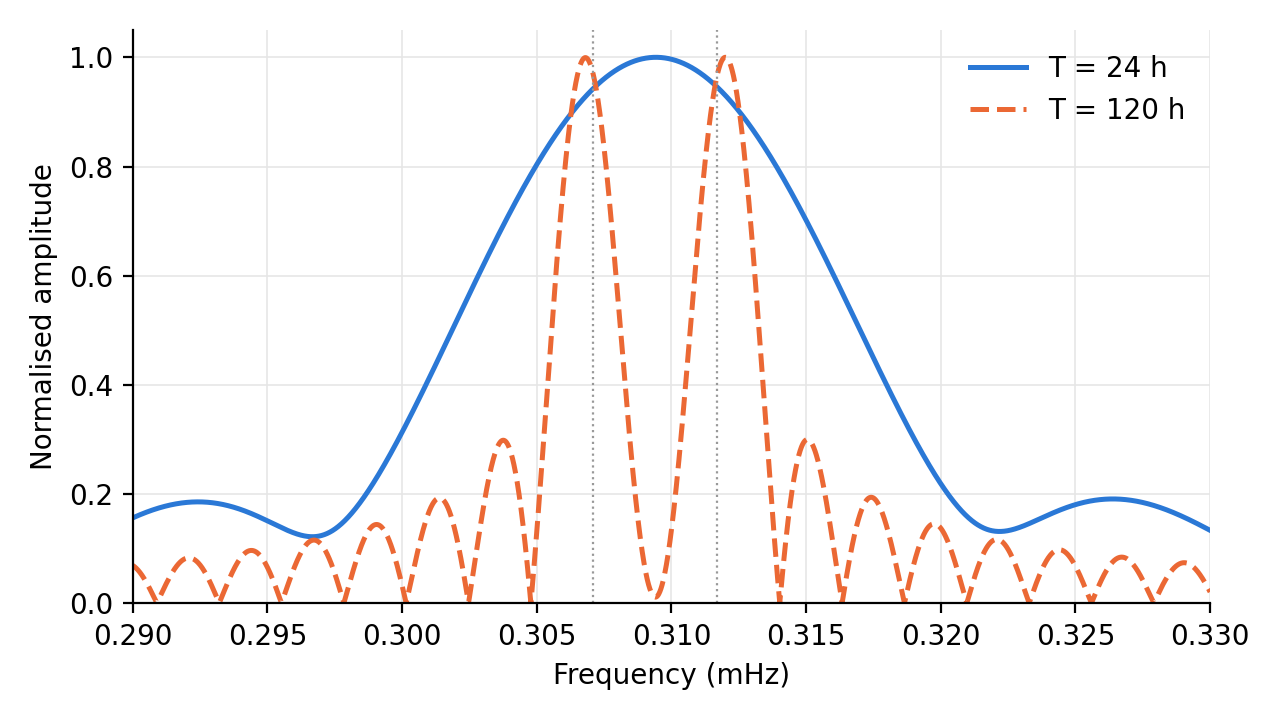
\includegraphics[width=0.7\textwidth]{figures_ex/ex11_window.png}
    \caption{Amplitude spectrum, normalised to its maximum, of the sum of two equal-amplitude cosines at
    the frequencies of two adjacent singlets of $_{0}S_{2}$ (dotted lines, separated by
    $4.6\,\mu\mathrm{Hz}$) observed through a boxcar window of length $24\,\mathrm{h}$ and $120\,\mathrm{h}$.
    Attenuation is neglected.}
    \label{fig:1}
\end{figure}

(c) With adjacent singlets $4.6\,\mu\mathrm{Hz}$ apart the criterion of part (b) requires
\begin{equation}
T\gtrsim\frac{1}{4.6\times 10^{-6}\,\mathrm{Hz}}=2.2\times 10^{5}\,\mathrm{s}\approx 60\,\mathrm{h},
\label{eq:31}
\end{equation}
that is, two and a half days. A one-day record has $1/T=11.6\,\mu\mathrm{Hz}$, larger than the width of
the entire multiplet ($4\times 4.6\approx 18\,\mu\mathrm{Hz}$), and shows a single broad peak, while a
five-day record has $1/T=2.3\,\mu\mathrm{Hz}$ and separates the singlets cleanly, as in Fig.~\ref{fig:1}.

Whether such records are available is set by attenuation. A mode with quality factor $Q$ decays as
$\ee^{-\omega_{0}t/2Q}=\ee^{-\pi f_{0}t/Q}$, so the amplitude $\ee$-folding time is
\begin{equation}
\tau=\frac{Q}{\pi f_{0}}=\frac{510}{\pi\times 3.094\times 10^{-4}\,\mathrm{s^{-1}}}=5.2\times 10^{5}\,\mathrm{s}\approx 6\,\mathrm{days}.
\label{eq:32}
\end{equation}
This is comfortably longer than the $60\,\mathrm{h}$ required: after five days the amplitude has fallen only
to $\ee^{-120/146}\approx 0.44$ of its initial value, so for a sufficiently large earthquake the signal
remains above the noise for long enough. Attenuation also sets a floor on the achievable resolution,
because the transform of $\ee^{-\pi f_{0}t/Q}\cos\omega_{0}t$ is a Lorentzian rather than a delta function,
with FWHM $f_{0}/Q\approx 0.6\,\mu\mathrm{Hz}$ in the power spectrum. Since this is well below the singlet
spacing, the splitting of $_{0}S_{2}$ is resolvable, and it is indeed observed after the very largest
earthquakes. Extending the record much beyond a few $\tau$ gains nothing, as the window then contains
mostly noise. The situation deteriorates at higher frequencies, where $f/Q$ grows to values comparable
with the widths of the multiplets, and this is why individual peaks become hard to identify in the
higher-frequency part of the spectrum shown in the lecture.
\end{solution}

%----------------------------------------------------------------------------------------
\begin{example}{Pointwise stability of an isotropic solid}
In an isotropic solid without pre-stress the elastic tensor is
$A_{ijkl}=\lambda\delta_{ij}\delta_{kl}+\mu(\delta_{ik}\delta_{jl}+\delta_{il}\delta_{jk})$.
(a)~For a complex symmetric tensor $e_{ij}$, decompose $e_{ij}$ into isotropic and deviatoric parts and
show that $A_{ijkl}e_{ij}^{*}e_{kl}=\kappa|e_{kk}|^{2}+2\mu\,d_{ij}^{*}d_{ij}$, where $d_{ij}$ is the
deviatoric part and $\kappa=\lambda+\frac{2}{3}\mu$. (b)~Show that the pointwise stability condition
$A_{ijkl}e_{ij}^{*}e_{kl}\ge c_{0}e_{ij}^{*}e_{ij}$ holds for some $c_{0}>0$ if and only if $\kappa>0$
and $\mu>0$, and find the largest admissible $c_{0}$. (c)~Show that these conditions imply
$\alpha>\beta>0$ for the P- and S-wave speeds, but that the converse fails, using $\lambda=-0.9\mu$ as a
counter-example. Explain physically why the two conditions differ.
\end{example}

\begin{solution}
(a) Write $e_{ij}$ as the sum of an isotropic part proportional to the identity and a traceless remainder,
\begin{equation}
e_{ij}=\tfrac{1}{3}\theta\,\delta_{ij}+d_{ij},\quad \theta=e_{kk},\quad d_{kk}=0.
\label{eq:33}
\end{equation}
The two parts are orthogonal: $\delta_{ij}d_{ij}=d_{kk}=0$, so that
\begin{equation}
e_{ij}^{*}e_{ij}=\tfrac{1}{9}|\theta|^{2}\delta_{ij}\delta_{ij}+d_{ij}^{*}d_{ij}
+\tfrac{1}{3}\left(\theta^{*}d_{kk}+\theta d_{kk}^{*}\right)=\tfrac{1}{3}|\theta|^{2}+d_{ij}^{*}d_{ij}.
\label{eq:34}
\end{equation}
Contracting the elastic tensor with $e_{ij}^{*}e_{kl}$, the $\lambda$ term gives
$\lambda\,e_{ii}^{*}e_{kk}=\lambda|\theta|^{2}$, and the two $\mu$ terms give
$\mu(e_{ij}^{*}e_{ij}+e_{ij}^{*}e_{ji})=2\mu\,e_{ij}^{*}e_{ij}$ by the symmetry of $e_{ij}$. Using
eq.~(\ref{eq:34}),
\begin{equation}
A_{ijkl}e_{ij}^{*}e_{kl}=\lambda|\theta|^{2}+2\mu\left(\tfrac{1}{3}|\theta|^{2}+d_{ij}^{*}d_{ij}\right)
=\kappa|\theta|^{2}+2\mu\,d_{ij}^{*}d_{ij},
\label{eq:35}
\end{equation}
with $\kappa=\lambda+\frac{2}{3}\mu$ the bulk modulus. The strain energy density
$\frac{1}{2}A_{ijkl}e_{ij}e_{kl}=\frac{1}{2}\kappa\theta^{2}+\mu\,d_{ij}d_{ij}$ thus splits into a part
that resists change of volume, governed by $\kappa$, and a part that resists change of shape, governed
by $\mu$.

(b) Combining eqs.~(\ref{eq:34}) and (\ref{eq:35}),
\begin{equation}
A_{ijkl}e_{ij}^{*}e_{kl}-c_{0}e_{ij}^{*}e_{ij}=(3\kappa-c_{0})\,\tfrac{1}{3}|\theta|^{2}+(2\mu-c_{0})\,d_{ij}^{*}d_{ij}.
\label{eq:36}
\end{equation}
If $c_{0}\le 3\kappa$ and $c_{0}\le 2\mu$ the right-hand side is non-negative for every symmetric
$e_{ij}$. Conversely, the choice $e_{ij}=\delta_{ij}$ (a pure dilatation, $\theta=3$, $d_{ij}=0$) makes the
right-hand side $3(3\kappa-c_{0})$, and a traceless choice such as $e_{12}=e_{21}=1$ with all other
components zero makes it $2(2\mu-c_{0})$, so both inequalities are also necessary. Pointwise stability
with some $c_{0}>0$ therefore holds if and only if $\kappa>0$ and $\mu>0$, and the largest admissible
constant is
\begin{equation}
c_{0}=\min(3\kappa,\,2\mu).
\label{eq:37}
\end{equation}
In other words, regarded as a symmetric linear map on the six-dimensional space of symmetric tensors,
$A_{ijkl}$ has the eigenvalue $3\kappa$ on the one-dimensional space of isotropic tensors and the
eigenvalue $2\mu$ on the five-dimensional space of deviatoric tensors, and $c_{0}$ is its smallest
eigenvalue.

(c) From the Christoffel equation in an isotropic material, $\rho\alpha^{2}=\lambda+2\mu=\kappa+\frac{4}{3}\mu$
and $\rho\beta^{2}=\mu$. If $\kappa>0$ and $\mu>0$ then $\beta^{2}>0$ and
$\rho(\alpha^{2}-\beta^{2})=\kappa+\frac{1}{3}\mu>0$, so $\alpha>\beta>0$. The converse fails: real
wave speeds with $\alpha>\beta$ require only $\mu>0$ and $\lambda>-2\mu$, whereas $\kappa>0$ requires the
stronger $\lambda>-\frac{2}{3}\mu$. For $\lambda=-0.9\mu$ with $\mu>0$ we have
\begin{equation}
\kappa=-0.9\mu+\tfrac{2}{3}\mu=-\tfrac{7}{30}\mu<0,\quad
\rho\alpha^{2}=1.1\mu>0,\quad \alpha=\sqrt{1.1}\,\beta\approx 1.05\beta,
\label{eq:38}
\end{equation}
so P- and S-waves propagate with real speeds and $\alpha>\beta>0$, yet the uniform dilatation
$e_{ij}=\delta_{ij}$ has $A_{ijkl}e_{ij}e_{kl}=9\kappa=-2.1\mu<0$ and the material is not pointwise stable.

The reason is that plane waves test the elastic tensor only on strains of a very special kind. A plane
wave with polarisation $\mathbf{a}$ and unit propagation direction $\hat{\mathbf{p}}$ produces the rank-one
strain $e_{ij}=\frac{1}{2}(a_{i}\hat{p}_{j}+a_{j}\hat{p}_{i})$, for which, using the symmetries of
$A_{ijkl}$, $A_{ijkl}e_{ij}e_{kl}=A_{ijkl}a_{i}\hat{p}_{j}a_{k}\hat{p}_{l}=\rho\,a_{i}\Gamma_{ik}(\hat{\mathbf{p}})a_{k}$
with $\Gamma_{ik}$ the Christoffel matrix. Such a strain has $\theta=\mathbf{a}\cdot\hat{\mathbf{p}}$ and
$e_{ij}e_{ij}=\frac{1}{2}[\|\mathbf{a}\|^{2}+(\mathbf{a}\cdot\hat{\mathbf{p}})^{2}]$, so by
eq.~(\ref{eq:34}) its deviatoric part satisfies
$d_{ij}d_{ij}=\frac{1}{2}\|\mathbf{a}\|^{2}+\frac{1}{6}(\mathbf{a}\cdot\hat{\mathbf{p}})^{2}$, and
eq.~(\ref{eq:35}) gives
\begin{equation}
A_{ijkl}e_{ij}e_{kl}=\mu\|\mathbf{a}\|^{2}+\left(\kappa+\tfrac{1}{3}\mu\right)(\mathbf{a}\cdot\hat{\mathbf{p}})^{2}
=\rho\left[\beta^{2}\|\mathbf{a}\|^{2}+(\alpha^{2}-\beta^{2})(\mathbf{a}\cdot\hat{\mathbf{p}})^{2}\right],
\label{eq:39}
\end{equation}
in agreement with the Christoffel matrix $\Gamma_{ik}=\alpha^{2}\hat{p}_{i}\hat{p}_{k}+\beta^{2}(\delta_{ik}-\hat{p}_{i}\hat{p}_{k})$
of Lecture~15. Even the longitudinal case $\mathbf{a}=\hat{\mathbf{p}}$ has $d_{ij}d_{ij}=\frac{2}{3}$
against $\frac{1}{3}\theta^{2}=\frac{1}{3}$: a rank-one strain is never a pure dilatation, and its
deviatoric part always outweighs its isotropic part. A sufficiently positive shear modulus can therefore
mask a negative bulk modulus in eq.~(\ref{eq:39}), which stays positive so long as
$\kappa>-\frac{4}{3}\mu$. A homogeneous compression, by contrast, has no deviatoric part at all; it is not
a plane wave of any finite wavelength, and it is precisely the strain that a negative $\kappa$ makes
energetically favourable.

The consequence for a finite body is decisive. Take $u_{i}=x_{i}$ on any body $M$ made of the material
in eq.~(\ref{eq:38}), so that $e_{ij}=\delta_{ij}$ everywhere and, in the non-gravitating case,
$\langle\mathbf{u}|H|\mathbf{u}\rangle=\int_{M}9\kappa\dd^{3}\mathbf{x}<0$. Expanding
$\mathbf{u}=\sum_{km}c_{km}|km\rangle$ with $c_{km}=\langle km|P|\mathbf{u}\rangle$, the eigenvalue
equation with test function $\mathbf{u}$ and the self-adjointness of $P$ give
\begin{equation}
\langle\mathbf{u}|H|\mathbf{u}\rangle=\sum_{km}c_{km}\langle\mathbf{u}|H|km\rangle
=\sum_{km}\omega_{k}^{2}c_{km}\langle\mathbf{u}|P|km\rangle=\sum_{km}\omega_{k}^{2}|c_{km}|^{2},
\label{eq:40}
\end{equation}
which can only be negative if at least one squared eigenfrequency is negative. The body therefore has a
mode that grows exponentially in time and is unstable, even though plane waves travel through the same
material perfectly well. Positive wave speeds are a condition on the propagation of disturbances of
finite wavelength; pointwise stability is the stronger condition that every strain, including a uniform
change of volume, costs energy, and it is the latter that the lecture needs to conclude that all the
squared eigenfrequencies of a non-gravitating earth model are non-negative.
\end{solution}

\end{document}
